\section{Algoritmo Genético}

\subsection{Orientações}

Foi requerida uma implementação de um Algoritmo Genético, onde fossem observados e descritos os seguintes critérios:

\begin{itemize}
	\item Utilizar obrigatoriamente a codificação binária
	\item Tamanho da população: 20.
	\item Seleção dos pais: escolhida pelo(a) projetista.
	\item Cruzamento: escolhido pelo(a) projetista.
	\item Taxa de cruzamento: 80\%.
	\item Mutação: escolhida pelo(a) projetista.
	\item Taxa de mutação: 3\%.
	\item Seleção de sobreviventes: elitista (os melhores indivíduos sempre sobrevivem).
	\item Critérios de parada: Número máximo de gerações alcançado: 1000; Se a solução ótima for encontrada.
	
	\item Apresentar a escolha e explicar o funcionamento dos operadores que foram utilizados: seleção dos pais, cruzamento e mutação.
	\item Execute 50 vezes o algoritmo e apresente, em forma de tabela, a	melhor solução encontrada em cada execução, o valor da função objetivo desta solução encontrada, o tempo de execução e o número da geração em que o algoritmo parou.
	\item Calcular a média e o desvio padrão do valor da função objetivo do melhor indivíduo, do tempo de execução e o número da geração em que o algoritmo parou (três últimas colunas da tabela).
	\item Mostre, pelo menos, duas soluções distintas encontradas pelo algoritmo.
	\item Comente e mostre o código fonte do algoritmo desenvolvido.
\end{itemize}

\subsection{Implementação}

Da mesma forma que no Hill Climbing, também foi utilizada a linguagem Python para a codificação deste algoritmo genético. Abaixo as bibliotecas utilizadas:

\lstinputlisting[name=ag,firstline=1, lastline=6]{../src/genetic-algorithm.py}

\subsubsection{Codificação da solução candidata}

Inicialmente, a codificação da solução candidata desse algoritmo é feita da mesma forma que no Hill Climbing, com uma lista contendo oito listas com 8 números aleatórios entre 0 e 7.

\lstinputlisting[name=ag, firstnumber=last,firstline=7, lastline=11]{../src/genetic-algorithm.py}

Como é necessário o uso da codificação binária para o cruzamento e mutação dos indivíduos, criou-se duas funções de transformação de binário para decimal e vice-versa.

\lstinputlisting[name=ag, firstnumber=last,firstline=12, lastline=20]{../src/genetic-algorithm.py}

A criação da população do algoritmo depende de um tamanho \verb|k|.

\lstinputlisting[name=ag, firstnumber=last,firstline=21, lastline=25]{../src/genetic-algorithm.py}

\subsubsection{Função Objetivo}

A função objetivo do Algoritmo Genético também é a mesma implementada no Hill Climbing. Portanto, o problema é configurado como sendo de minimização.

\lstinputlisting[name=ag, firstnumber=last,firstline=26, lastline=59]{../src/genetic-algorithm.py}

\subsubsection{Operadores}

A \textbf{seleção dos pais} se deu pela estratégia da roleta. Ao receber como argumentos uma população e a lista de fitness de cada indivíduo, a função \verb*|select_parents()| divide a fitness de cada indivíduo pela soma todos os valores de fitness, obtendo assim uma distribuição de probabilidades. \verb*|numpy.random.choice| escolhe dois números de acordo com a distribuição, sem reposição. Assim, os dois números servem como os índices de dois indivíduos na população que são escolhidos como pais da geração atual.

\lstinputlisting[name=ag, firstnumber=last,firstline=60, lastline=71]{../src/genetic-algorithm.py}

O \textbf{cruzamento} dos pais escolhidos depende de uma taxa de cruzamento \verb*|cross_rate|. Caso um número aleatório entre 0 e 1 seja menor que \verb*|cross_rate| o cruzamento acontece. A troca de material genético é feita através da estratégia do ponto de corte, onde os pais são seccionados em duas partes, gerando filhos por meio da combinação dessas partes. Se o cruzamento não acontecer, os pais se tornam os filhos.

\lstinputlisting[name=ag, firstnumber=last,firstline=72, lastline=92]{../src/genetic-algorithm.py}

A \textbf{mutação} dos filhos também possui uma probabilidade de acontecer. Caso um número aleatório entre 0 e 1 seja menor que a taxa de mutação \verb*|mutate_rate| a mutação é realizada. A estratégia do bit flip consiste em trocar um dos 24 bits que representam a solução pelo seu inverso. Caso a mutação não ocorra, o filho permanece inalterado

\lstinputlisting[name=ag, firstnumber=last,firstline=93, lastline=120]{../src/genetic-algorithm.py}

A seleção dos sobreviventes é feita de forma elitista, onde apenas os \verb*|k| indivíduos com a menor fitness sobrevivem para a próxima geração. A fim de ordenar a lista de indivíduos em ordem crescente pela sua respectiva fitness, a função \verb*|select_survivors| recebe um mapeamento entre esses dois parâmetros, facilitando a ordenação e o corte.

\lstinputlisting[name=ag, firstnumber=last,firstline=121, lastline=126]{../src/genetic-algorithm.py}

Com a geração da população em mãos, além dos operadores genéticos, o algoritmo genético foi estruturado para receber os valores de \verb*|k| indivíduos da população, a taxa de crossover \verb*|cross_rate|, a taxa de mutação \verb*|mutate_rate| e o número máximo de gerações \verb*|gen|.

Ao iniciar a população original e calcular a fitness dos indivíduos, uma variável \verb*|best_solution| passa a armazenar a tupla que representa a solução com a menor fitness.

Em seguida, um laço é executado até que um dos seguintes critérios de parada seja atendido:
\begin{itemize}
	\item Uma indivíduo com fitness igual a zero seja encontrado.
	\item O número de gerações passe do que foi estipulado por \verb*|gen|.
\end{itemize}

Dentro do laço são aplicados os operadores genéticos de seleção dos pais, cruzamento, mutação e seleção dos sobreviventes. Ao fim das iterações, a solução com o menor fitness assume o posto de melhor solução. São retornados a melhor solução, sua fitness e a diferença ente o número máximo de gerações e a quantidade de gerações necessárias para para o algoritmo.

\lstinputlisting[name=ag, firstnumber=last,firstline=127, lastline=166]{../src/genetic-algorithm.py}

\subsection{Execução e Análise de resultados}

\subsubsection{Execução}

A fim de armazenar alguns dados das 50 execuções pedidas, foram criadas quatro listas \verb*|166:172|:
\begin{itemize}
	\item \verb*|execution|: armazena os índices das 50 execuções
	\item \verb*|solutions|: armazena as soluções das 50 execuções
	\item \verb*|fitnesses|: armazena os valores de fitness das 50 soluções
	\item \verb*|generations|: armazena o número de gerações necessárias para as 50 execuções
	\item \verb*|runtimes|: armazena o tempo de execução de cada uma das 50 execuções. O cálculo do tempo foi feito através da diferença entre o tempo da CPU antes e depois da execução do Algoritmo Genético.
\end{itemize}

\lstinputlisting[name=ag, firstnumber=last,firstline=166, lastline=185]{../src/genetic-algorithm.py}

Executando essas instruções, foram obtidos os seguintes dados:

\begin{figure}[H]
	\centering
	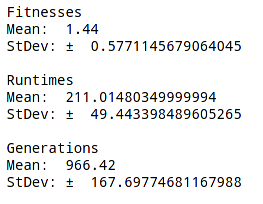
\includegraphics[scale=.7]{img/stats_ag}
	\caption{Média e desvio padrão de iterações e runtimes de 50 execuções}
	\label{statsag}
\end{figure}

O seguinte dataframe organiza as informações obtidas em um formato de tabela.

\lstinputlisting[name=ag, firstnumber=last,firstline=186, lastline=192]{../src/genetic-algorithm.py}

\begin{figure}[H]
	\centering
	\begin{subfigure}{.5\textwidth}
		\centering
		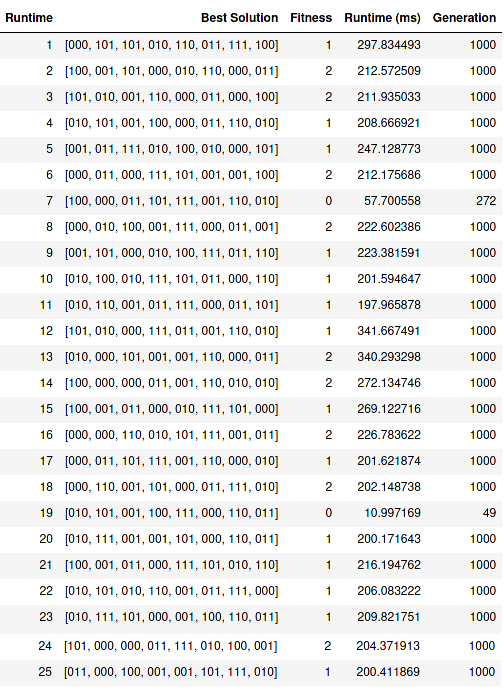
\includegraphics[scale=.5]{img/df1}
		\caption{25 primeiras execuções}
	\end{subfigure}%
	\begin{subfigure}{.5\textwidth}
		\centering
		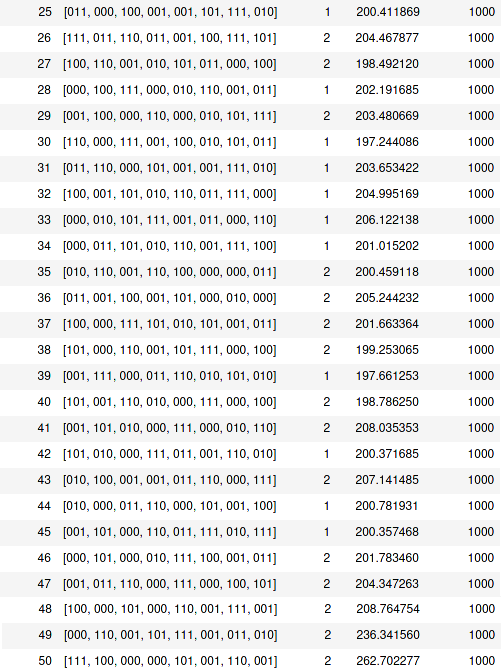
\includegraphics[scale=.5]{img/df2}
		\caption{25 últimas execuções}
	\end{subfigure}%
\end{figure}



\subsubsection{Melhores soluções encontradas}

As 5 melhores soluções obtidas para a mesma execução da figura (\ref{statsag}) foram separadas e exibidas.

\lstinputlisting[name=ag, firstnumber=last,firstline=215, lastline=231]{../src/genetic-algorithm.py}

\begin{verbatim}
	----------------------------------
	Solution:  ['010', '101', '001', '100', '111', '000', '110', '011']
	Fitness:  0
	----------------------------------
	Solution:  ['100', '000', '011', '101', '111', '001', '110', '010']
	Fitness:  0
	----------------------------------
	Solution:  ['000', '010', '101', '111', '001', '011', '000', '110']
	Fitness:  1
	----------------------------------
	Solution:  ['000', '011', '101', '010', '110', '001', '111', '100']
	Fitness:  1
	----------------------------------
	Solution:  ['000', '011', '101', '111', '001', '110', '000', '010']
	Fitness:  1
\end{verbatim}